%!TEX root = ../thesis.tex

\section{実験1}
\subsection{実験目的}
シミュレータ上で実験を行い, 提案手法の有効性を検証する.

\subsection{実験装置}
実験は, \figref{Fig:gazebo}に示すGazebo\cite{gazebo}のWillow Garage\cite{willow}で\figref{Fig:willow-garage}に示すコースで一周行う. また, ロボットモデルには\figref{Fig:turtlebot3}に示すようなカメラを3つ搭載したTurtlebot3\cite{turtlebot3}を用いた. 

\begin{figure}[h]
  \centering
  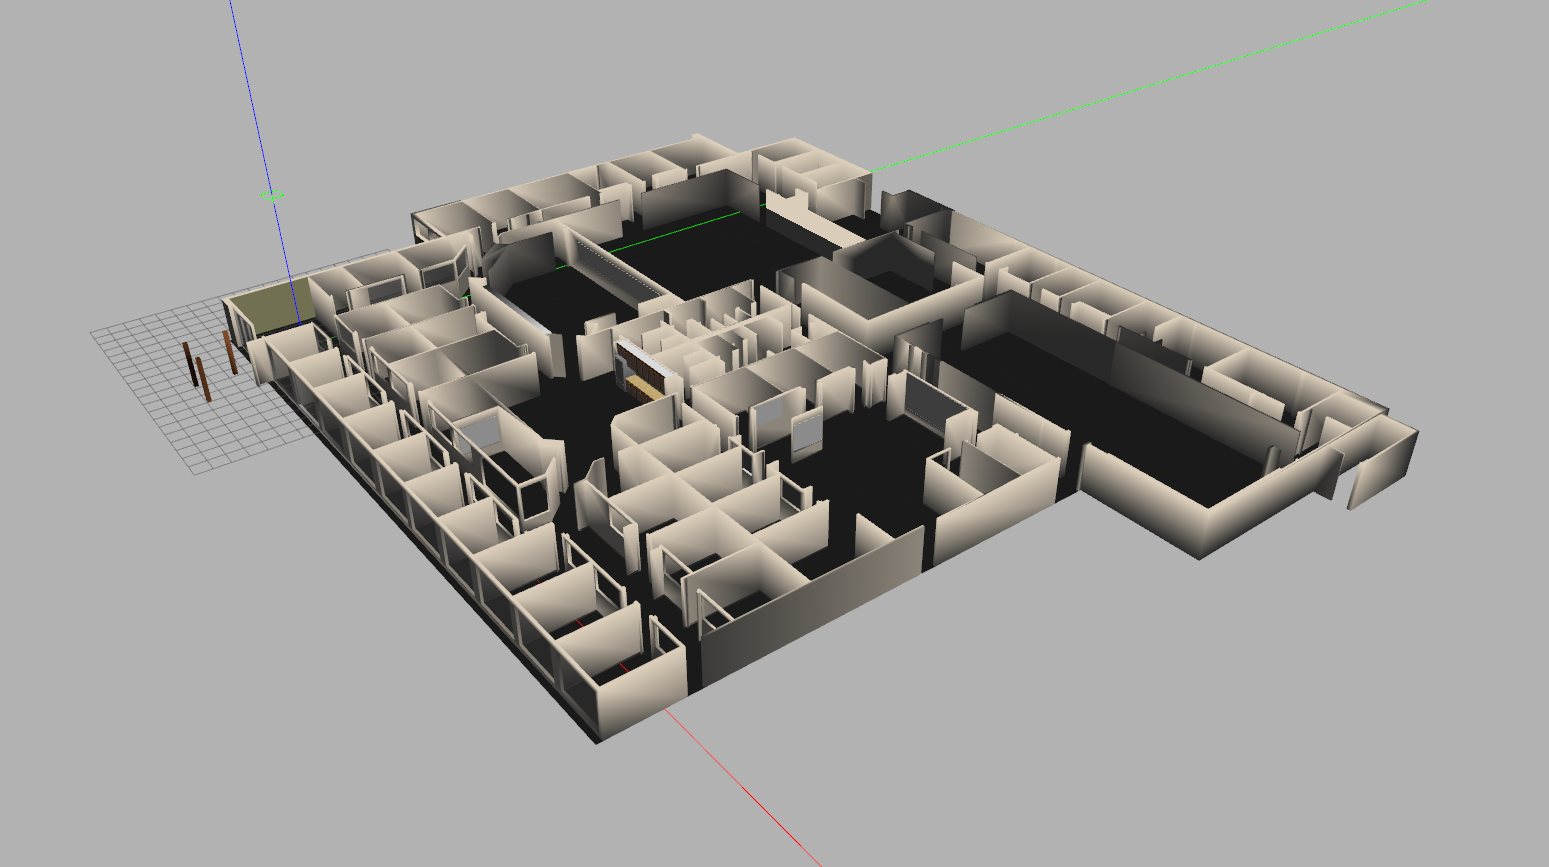
\includegraphics[keepaspectratio, scale=0.15]{images/gazebo.png}
  \caption{Experimental environment in simulator}
  \label{Fig:gazebo}
  \end{figure}

\begin{figure}[h]
  \centering
  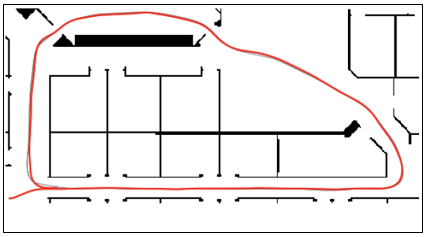
\includegraphics[keepaspectratio, scale=0.5]{images/willow-garage.png}
  \caption{Course to collect data}
  \label{Fig:willow-garage}
  \end{figure}

\begin{figure}[h]
  \centering
  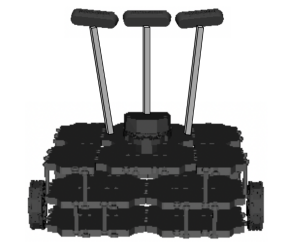
\includegraphics[keepaspectratio, scale=0.55]{images/turtlebot3.png}
  \caption{Turtlebot3 waffle with 3 cameras}
  \label{Fig:turtlebot3}
  \end{figure}

\newpage
\subsection{実験方法}
\begin{description}
  \item[1.データ収集フェーズ]\mbox{}\\データの収集方法について述べる. \figref{Fig:old-method}にデータの収集方法を示す. 赤色の線である目標経路から平行に±0.10, ±0.20, ±0.30m離れた座標にロボットを配置する. そして, その座標ごとに目標経路に沿った向きを基準として±5度傾けて, カメラ画像とナビゲーションの出力である角速度を収集する. これを\figref{Fig:willow-garage}に示した経路で実験を行う. 
\end{description}

\begin{figure}[h]
  \centering
  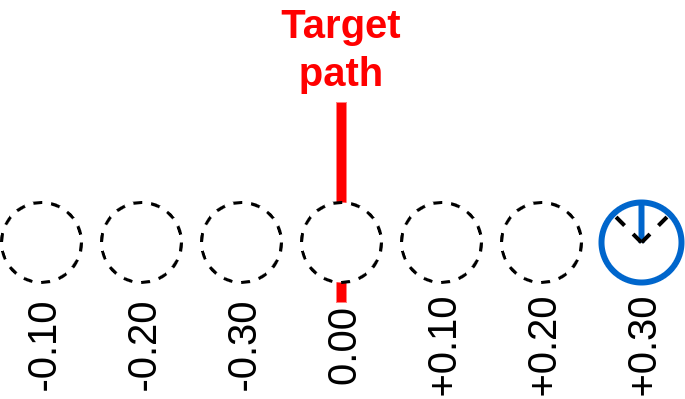
\includegraphics[keepaspectratio, scale=0.25]{images/old-method.png}
  \caption{Method of collecting data around the target route}
  \label{Fig:old-method}
  \end{figure}

\newpage
\begin{description}
  \item[2.訓練フェーズ]\mbox{}\\データ量2748, 従来手法とバッチ学習それぞれで4000step, 8000step, 10000step学習した. なお, 4000stepは従来研究において, シミュレータの実験に用いられてきたステップ数であり, 10000stepは従来研究において, 実ロボットの実験に用いられていたステップ数である. 
\end{description}

\begin{description}
  \item[3.テストフェーズ]\mbox{}\\ \figref{Fig:willow-garage}に示すコースで10回走行させる. ロボットの並進速度0.2m/sとし, 経路を3周できた場合を成功, 壁に激突したり, 経路から10m離れたりした場合を失敗とした.
\end{description}

\subsection{実験結果}
実験結果を表\ref{tb:exp1.1}, \ref{tb:exp1.2}に示す. また, 失敗箇所は\figref{Fig:result1.1}, \figref{Fig:result1.2}, 失敗箇所ごとの失敗回数は表\ref{tb:fail1.1}, \ref{tb:fail1.2}のようになった. 

\newpage
\begin{description}
  \item [(1)従来手法]
\end{description}

\begin{table}[h]
  \centering
  \begin{tabular}{|c|c|} \hline
    Experiments & Number of successes \\ \hline
    Exp.1(4000step) & 0/5 \\ \hline
    Exp.2(8000step) & 0/5 \\ \hline
    Exp.3(10000step) & 0/5 \\ \hline
  \end{tabular}
  \caption{Number of successes in the conventional method}
  \label{tb:exp1.1}
\end{table}

\begin{figure}[h]
  \centering
  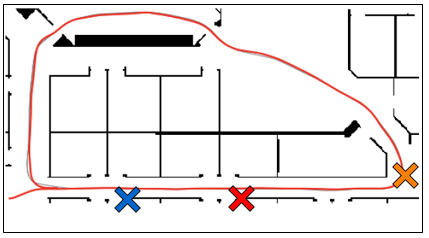
\includegraphics[keepaspectratio, scale=0.5]{images/result1.png}
  \caption{Failure point of the experiment}
  \label{Fig:result1.1}
  \end{figure}

\begin{table}[h]
  \centering
  \begin{tabular}{|c|c|c|} \hline
    Experiments & Number of failures with red x & Number of failures with blue x \\ \hline
    Exp.1(4000step) & 0 & 5 \\ \hline
    Exp.2(8000step) & 0 & 5 \\ \hline
    Exp.3(10000step) & 1 & 4 \\ \hline
  \end{tabular}
  \caption{Number of failures in the experiment}
  \label{tb:fail1.1}
\end{table}

\newpage
\begin{description}
  \item [(2)バッチ学習]
\end{description}

\begin{table}[h]
  \centering
  \begin{tabular}{|c|c|} \hline
    Experiments & Number of successes \\ \hline
    Exp.1(4000step) & 0/1 \\ \hline
    Exp.2(8000step) & 0/1 \\ \hline
    Exp.3(10000step) & 0/1 \\ \hline
  \end{tabular}
  \caption{Number of successes in the batch learning}
  \label{tb:exp1.2}
\end{table}

\begin{figure}[h]
  \centering
  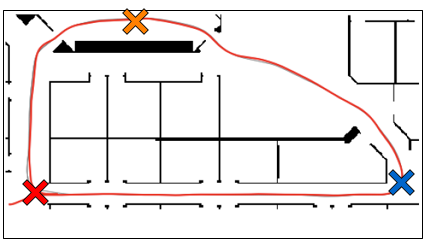
\includegraphics[keepaspectratio, scale=0.5]{images/result1.2.png}
  \caption{Failure point of the experiment}
  \label{Fig:result1.2}
  \end{figure}

\begin{table}[h]
  \centering
  \begin{tabular}{|c|c|c|} \hline
    Experiments & Number of failures with blue x \\ \hline
    Exp.1(4000step) & 1 \\ \hline
    Exp.2(8000step) & 1 \\ \hline
    Exp.3(10000step) & 1 \\ \hline
  \end{tabular}
  \caption{Number of failures in the experiment}
  \label{tb:fail1.2}
\end{table}

\newpage
\subsection{考察}
従来手法では直進時, 経路から離れた際に経路に戻る挙動や, 壁に近づいた際に避ける挙動が見られなかった. これは, 訓練時に全てのデータを使用せずに, 直進のデータをいくつか捨ててしまっているためだと考えられる. また, バッチ学習では, 訓練時に全てのデータを使用しているため, 壁に衝突することなく直進できたと考えられる. しかし, \figref{Fig:result1.2}の青×の箇所で角を曲がり切ることができずにコースアウトしてしまった. ここで, 訓練させた際のlossを以下に示す. 従来手法の\figref{Fig:exp1.1_4000}, \figref{Fig:exp1.1_8000}, \figref{Fig:exp1.1_10000}は正しく学習できず, オーバシュートしている. バッチ学習の\figref{Fig:exp1.2_4000}, \figref{Fig:exp1.2_8000}, \figref{Fig:exp1.2_10000}では. ステップ数を増やすに連れて学習が収束していることが分かる. 角を曲がりきれなかった要因の一つとして, コースアウトした箇所付近の目標経路周辺のデータが足りないためだと考えられる. そこで, 次に目標経路と平行な方向のロボット配置間隔を狭めて, データ量を増やすことで成功回数が増えるか検証する. 
% ステップ数を増やしても成功回数は増えなかった.  また, 目標経路から離れた際に戻る挙動や, 壁に近づきすぎた際に避ける挙動も見られなかった. ここで, 訓練させた際の各実験ごとのlossを\figref{Fig:exp1-4000}, \figref{Fig:exp1-8000}, \figref{Fig:exp1-10000}に示す. 4000stepから10000step全てにおいて, オーバーシュートしていると考えられる. そこで, 収集した角速度を\figref{Fig:exp1}のようにヒストグラムにした. これより, 経路上及び経路周辺のデータである0.0rad/sから0.1rad/sが全体の40\%程度しかないことが分かる. 以上を踏まえて, 経路上及び経路周辺のデータが多い方が, 経路追従できるのではないかと考えた. 

\newpage
\begin{figure}[h]
  \centering
  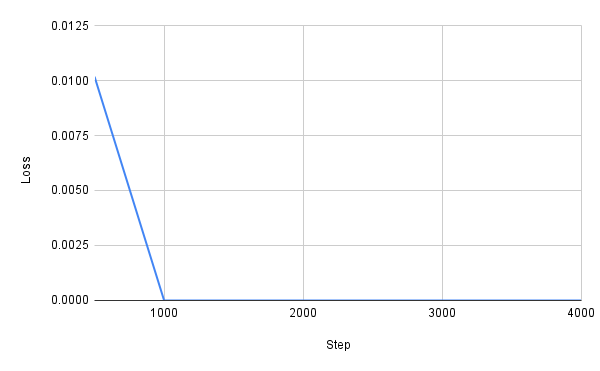
\includegraphics[keepaspectratio, scale=0.31]{images/exp1.1_4000.png}
  \caption{Loss value in the experiment1}
  \label{Fig:exp1.1_4000}
  \end{figure}

\begin{figure}[h]
  \centering
  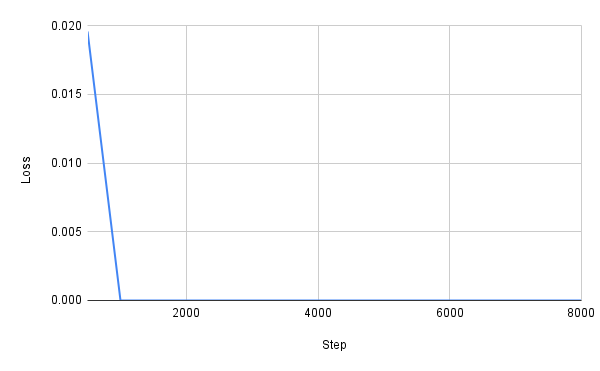
\includegraphics[keepaspectratio, scale=0.31]{images/exp1.1_8000.png}
  \caption{Loss value in the experiment2}
  \label{Fig:exp1.1_8000}
  \end{figure}

\begin{figure}[h]
  \centering
  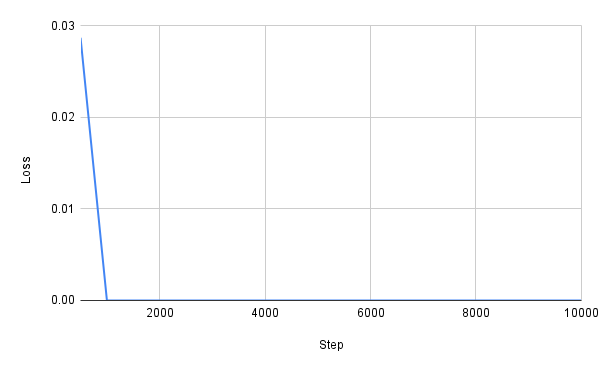
\includegraphics[keepaspectratio, scale=0.31]{images/exp1.1_10000.png}
  \caption{Loss value in the experiment3}
  \label{Fig:exp1.1_10000}
  \end{figure}

\newpage
\begin{figure}[h]
  \centering
  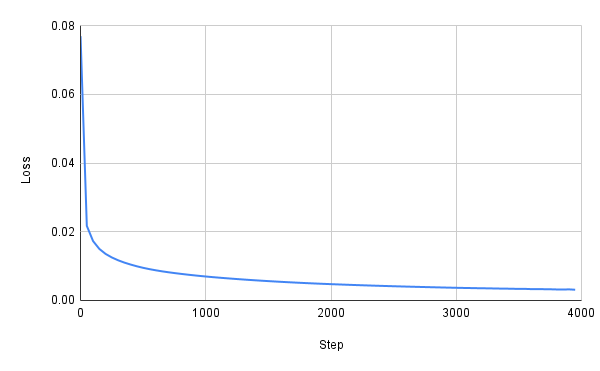
\includegraphics[keepaspectratio, scale=0.31]{images/exp1.2_4000.png}
  \caption{Loss value in the experiment1}
  \label{Fig:exp1.2_4000}
  \end{figure}
  
\begin{figure}[h]
  \centering
  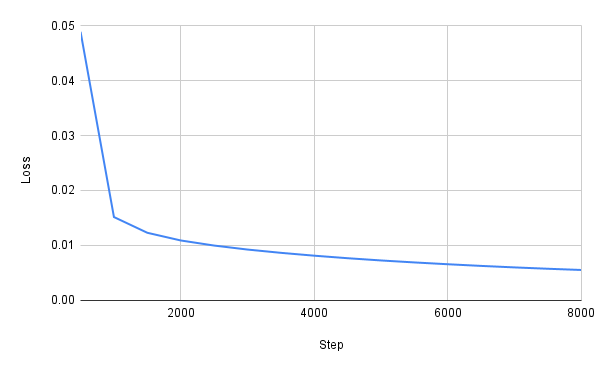
\includegraphics[keepaspectratio, scale=0.31]{images/exp1.2_8000.png}
  \caption{Loss value in the experiment2}
  \label{Fig:exp1.2_8000}
  \end{figure}

\begin{figure}[h]
  \centering
  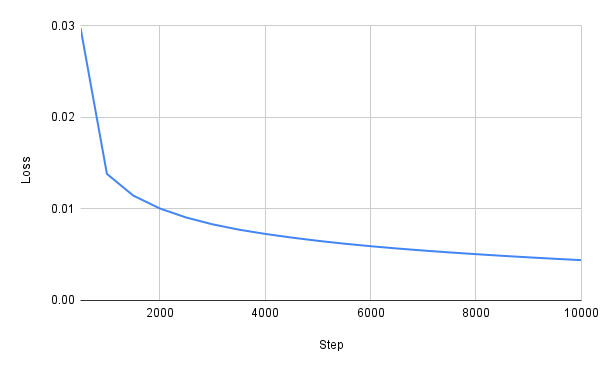
\includegraphics[keepaspectratio, scale=0.31]{images/exp1.2_10000.png}
  \caption{Loss value in the experiment3}
  \label{Fig:exp1.2_10000}
  \end{figure}

\newpage
\section{実験2}
実験目的, 実験装置, テストフェーズは実験1と同様である.
\subsection{実験方法}
\begin{description}
  \item[1.データ収集フェーズ]\mbox{}\\実験1を踏まえて, 経路周辺のデータを多く取得する手法を試みる. \figref{Fig:collect-data}にデータの収集方法を示す. 赤色の線である目標経路から平行に±0.01, ±0.02, ±0.04, ±0.06, ±0.08, ±0.10, ±0.15, ±0.20, ±0.30m離れた座標にロボットを配置する. そして, 手法1と同様にロボットを傾けて画像と角速度を\figref{Fig:collect-data2}のように収集する. これを\figref{Fig:willow-garage}に示すコースで一周行う.  
\end{description}

\begin{figure}[h]
  \centering
  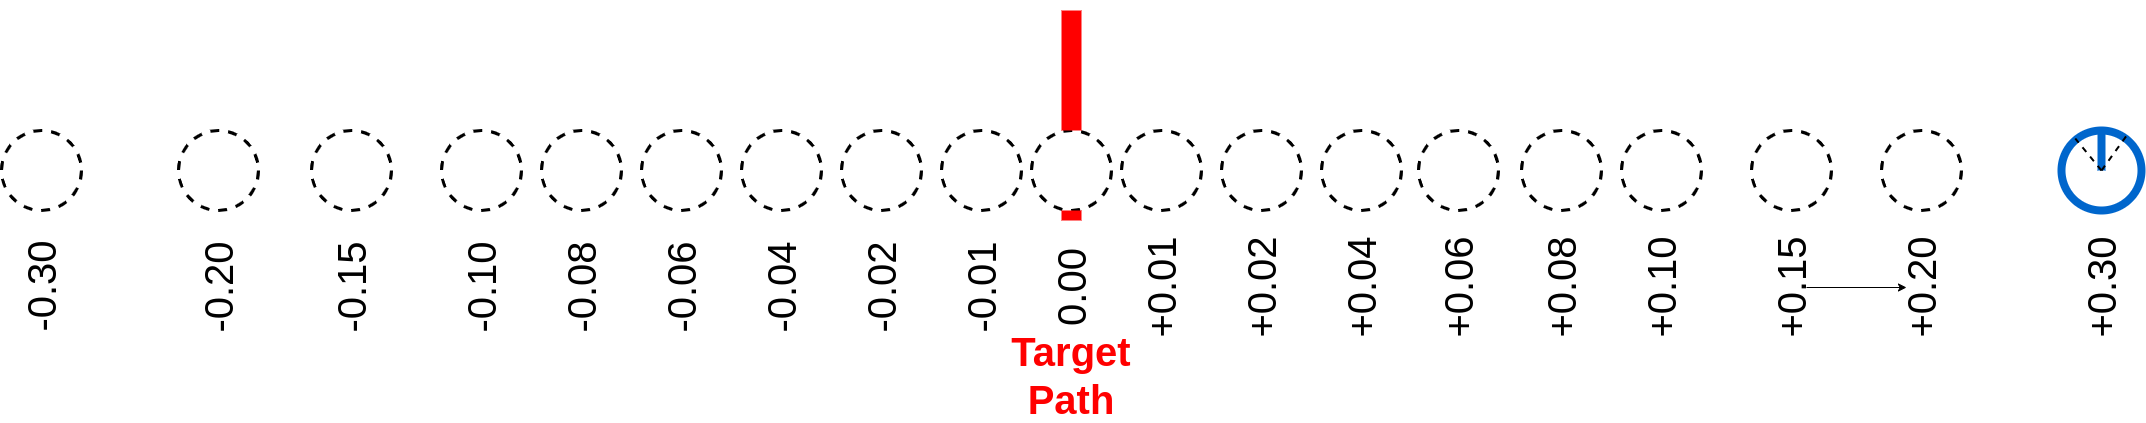
\includegraphics[keepaspectratio, scale=0.18]{images/collect-data.png}
  \caption{Method of collecting data around the target route}
  \label{Fig:collect-data}
  \end{figure}

\begin{description}
  \item[2.訓練フェーズ]\mbox{}\\データ量7452, 従来手法とバッチ学習それぞれで4000step, 8000step, 10000step学習した. 
\end{description}

\subsection{実験結果}
実験結果を表\ref{tb:exp2}, \ref{tb:exp3}に示す. また, 失敗箇所は\figref{Fig:result2}, 失敗箇所ごとの失敗回数は表\ref{tb:fail2}であった. 

\newpage
\begin{description}
  \item [(1)従来手法]
\end{description}
\begin{table}[h]
  \centering
  \begin{tabular}{|c|c|} \hline
    Experiments & Number of successes \\ \hline
    Exp.1(4000step) & 0/5 \\ \hline
    Exp.2(8000step) & 0/5 \\ \hline
    Exp.3(10000step) & 0/5 \\ \hline
  \end{tabular}
  \caption{Number of successes in the experiment}
  \label{tb:exp2}
\end{table}

\begin{figure}[h]
  \centering
  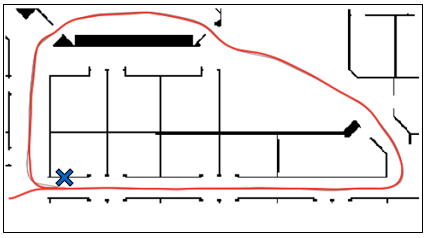
\includegraphics[keepaspectratio, scale=0.5]{images/result2.png}
  \caption{Failure point of the experiment2-1}
  \label{Fig:result2}
  \end{figure}

\begin{table}[h]
  \centering
  \begin{tabular}{|c|c|c|} \hline
    Experiments & Number of failures with blue x \\ \hline
    Exp.1(4000step) & 5 \\ \hline
    Exp.2(8000step) & 5 \\ \hline
    Exp.3(10000step) & 5 \\ \hline
  \end{tabular}
  \caption{Number of failures in the experiment}
  \label{tb:fail2}
\end{table}

\newpage
\begin{table}[h]
  \centering
  \begin{tabular}{|c|c|} \hline
    Experiments & Number of successes \\ \hline
    Exp.1(4000step) & 10/10 \\ \hline
    Exp.2(8000step) & 10/10 \\ \hline
    Exp.3(10000step) & 10/10 \\ \hline
  \end{tabular}
  \caption{Number of successes in the experiment3}
  \label{tb:exp3}
\end{table}

\subsection{考察}
実験1と実験2で収集した角速度のデータ量の比率を\figref{Fig:hist}に示す. 実験2では, 収集したデータ量全体の数も増えているが, 角を曲がる際の角速度0.3rad/s以上のデータも増えていることが分かる. また, 従来手法では, 4000step, 8000step, 10000step全てで\figref{Fig:result2}の青×に示す箇所で壁に衝突して失敗した. 実験1の\figref{Fig:result1.1}と比べて走行距離が短くなっているのは, 角のデータが増えたが, 訓練時に全てのデータを使用していないため, 左折する行動を学習してしまったためだと考えられる. 実験2では, 4000step, 8000step, 10000step全てで成功回数が10/10となり, 経路を周回することができた. このことから, 目標経路周辺においてロボットの配置間隔を狭め, バッチ学習を用いて訓練することで経路追従できることを確認した. 
% 収集した角速度を\figref{Fig:exp2}のようにヒストグラムにした. 経路上及び経路周辺のデータである0.0rad/sから0.1rad/sが全体の68.3\%になり, \figref{Fig:exp1}と比べて多くなっている. また, 4000step, 8000step, 10000step全て\figref{Fig:result2}に青×の箇所で壁に衝突し失敗した. 結果として, 経路上や経路周辺のデータを増やしたり, ステップ数を増やしたりしても成功回数は増えなかった. ここで, 訓練させた際の各実験ごとのlossを\figref{Fig:exp2-4000}, \figref{Fig:exp2-8000}, \figref{Fig:exp2-10000}に示す. 実験1と同様に4000stepから10000step全てにおいて, オーバーシュートしていると考えられる. 先行研究では, オンラインで学習を行うため, 計算のリソースなどの観点からバッチサイズを8にしていた. しかし, 提案手法ではオフラインで学習を行うため, バッチ学習に変更する. これにより, 一度に大量のデータを扱えるため最適解に辿り着くことができ, 成功回数が増えるのではないかと考えた. 

\begin{figure}[h]
  \centering
  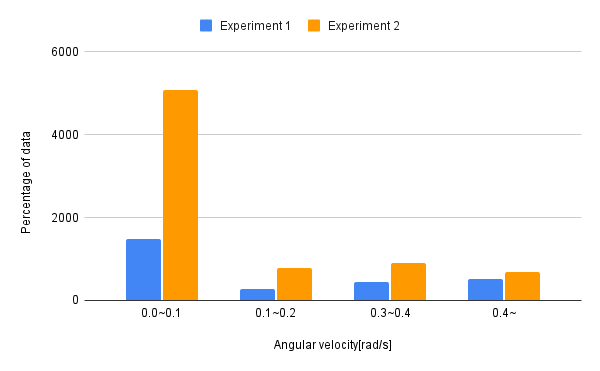
\includegraphics[keepaspectratio, scale=0.4]{images/ang_sum.png}
  \caption{Histogram of collected angular velocities in the experiment1 and the experiment2}
  \label{Fig:hist}
  \end{figure}

\newpage
\begin{figure}[h]
  \centering
  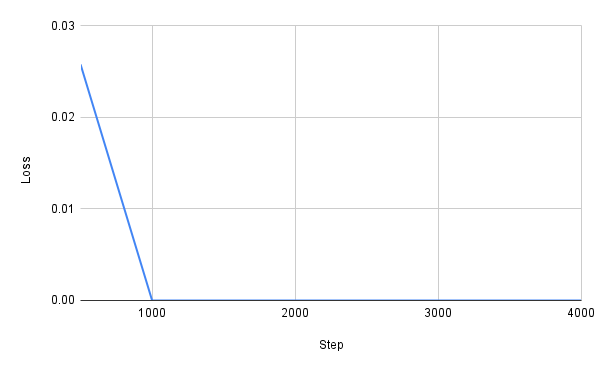
\includegraphics[keepaspectratio, scale=0.31]{images/exp2_4000.png}
  \caption{Loss value in the experiment1}
  \label{Fig:exp2-4000}
  \end{figure}

\begin{figure}[h]
  \centering
  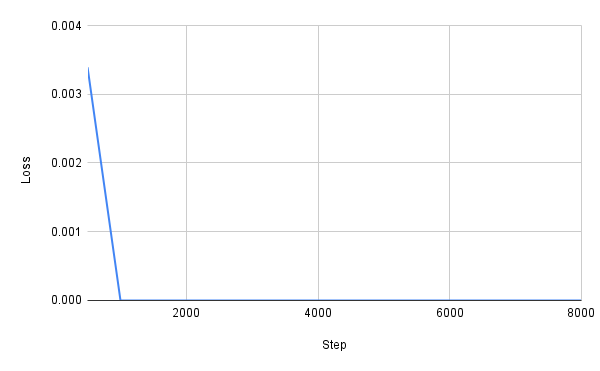
\includegraphics[keepaspectratio, scale=0.31]{images/exp2_8000.png}
  \caption{Loss value in the experiment2}
  \label{Fig:exp2-8000}
  \end{figure}

\begin{figure}[h]
  \centering
  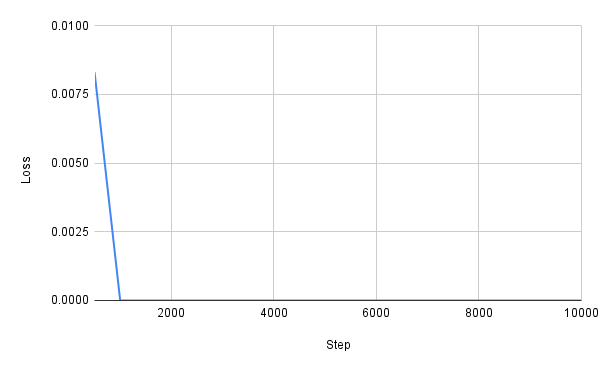
\includegraphics[keepaspectratio, scale=0.31]{images/exp2_10000.png}
  \caption{Loss value in the experiment3}
  \label{Fig:exp2-10000}
  \end{figure}
  
\newpage
\begin{figure}[h]
  \centering
  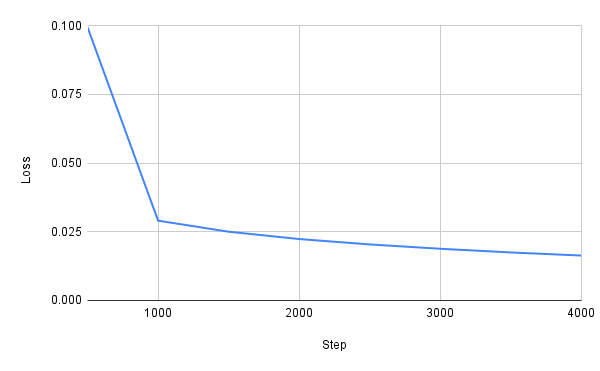
\includegraphics[keepaspectratio, scale=0.31]{images/exp3_4000.png}
  \caption{Loss value in the experiment1}
  \label{Fig:exp3-4000}
  \end{figure}

\begin{figure}[h]
  \centering
  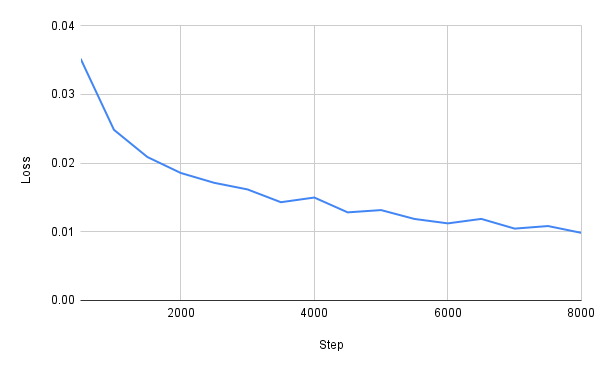
\includegraphics[keepaspectratio, scale=0.31]{images/exp3_8000.png}
  \caption{Loss value in the experiment2}
  \label{Fig:exp3-8000}
  \end{figure}

\begin{figure}[h]
  \centering
  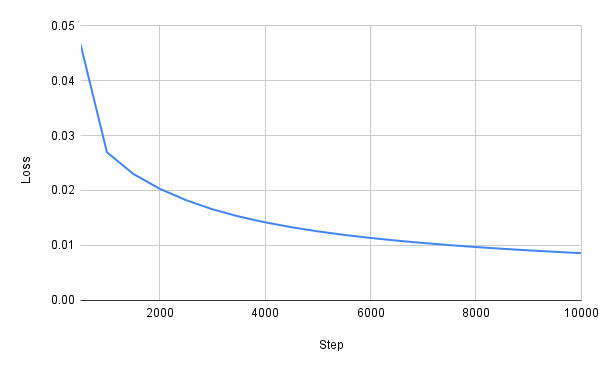
\includegraphics[keepaspectratio, scale=0.31]{images/exp3_10000.png}
  \caption{Loss value in the experiment3}
  \label{Fig:exp3-10000}
  \end{figure}